% importa variabili globali
% definizione variabili globali
\def\GRUPPO {\textit{DazzleWorks}}

\def\PROGETTO {\textbf{Premi}}

\def\COMMITTENTE {Prof. Vardanega Tullio, \\ & Dr. Cardin Riccardo}

\def\EMAIL {dazzleworksgroup@gmail.com}

\def\LOGO {../../template/img/logo.png}

\def\INTESTAZIONE {../../template/img/intestazione.png}
\def\PIEDIPAGINA {../../template/img/piedipagina.png}

\def\G {{\small $_G$}}


% definizione variabili locali
\def\DOCUMENTO{Manuale Utente}
\def\VERSIONE{2.0.0}

\def\DESCRIZIONE{Documento che facilita l'utilizzo dell'applicazione da parte dell'utente.}

\def\REDATTORE {Suierica Bogdan}
\def\VERIFICATORE {Ros Fabio}
\def\RESPONSABILE {Agostinetto Matteo}

\def\USO {Esterno}

\def\DISTRIBUZIONE {\GRUPPO{}\\ & \COMMITTENTE{}\\ & \PROPONENTE{}\\}


% abilita (true) / disabilita (false) indice, lista tabelle, lista figure
\def\INDICE	{true}
\def\TABELLE {true}
\def\FIGURE {true}


% importa struttura
\documentclass[a4paper]{article}

% ----- definizioni -----
\def\TITLE		{\mbox{\GRUPPO}}
\def\SUBTITLE	{\SIGLA, \PROGETTO}


% ----- nuovi comandi -----
% fornisce il caption per riferirsi ad una particolare sezione
\newcommand{\numref}[1]{\textsf{\textsl{``\nameref{#1}'' (\ref{#1})}}}


% ----- package -----
\usepackage[T1]{fontenc}   % codifica dei font in uscita
\usepackage[utf8x]{inputenc}   % lettere accentate da tastiera
\usepackage[italian]{babel}   % lingua principale del documento
\usepackage[a4paper, top= 3cm, bottom= 3cm, left= 3cm, right= 3cm, bindingoffset= 5mm]{geometry} % impostazione margini

\usepackage{amssymb} %

\usepackage{booktabs} % comandi aggiuntivi per le tabelle

\usepackage{calc} % espressioni aritmetiche
\usepackage{caption} % descrizione figure, ecc
\usepackage{chapterbib} % inclusione delle bibliografie

\usepackage{datatool} % manipolazione dati
\usepackage{dcolumn} % array in tabular

\usepackage{epstopdf} % conversione eps--> pdf
\usepackage{enumitem} % personalizzazione liste
\usepackage{eurosym} % simbolo euro

\usepackage{fancyhdr}   %personalizzazione dello stile
\usepackage{float} % definizione di oggetti floating (es. figure, tabelle)
\usepackage[bottom]{footmisc} % personalizzazione note

\usepackage[toc]{glossaries}	% glossario
\usepackage{graphicx, subfigure} % pacchetto grafica testo
\usepackage{grffile} % estende gestione filename graphic

\usepackage[colorlinks=true, urlcolor=blue, citecolor=black, linkcolor=black, hyperindex, breaklinks]{hyperref} % gestione dei link

\usepackage{ifthen}	% costrutto ifthenelse

% \usepackage{listings} % inserimento pezzi di codice
\usepackage{longtable} % tabelle su più pagine

\usepackage{pgf} % grafica postscript e PDF
\usepackage{pgfplots}	% composizione di grafici
\pgfplotsset{/pgf/number format/use comma, compat=newest}	% opzioni per i grafici

\usepackage{multirow} % span multiriga

\usepackage{tabularx, array} % crea paragrafi a colonne
\usepackage{titlesec} % personalizzazione titoli
\usepackage{tikz} % gestione delle formule
\usepackage{totpages} % conta numero pagine

\usepackage{soul} % gestione letterspacing
\usepackage{subfigure} % gestione delle sottofigure

\usepackage{verbatim} % inserimento testo verbatim, non interpretato

\usepackage{wallpaper} % gestione background

\usepackage{xspace} % spazi automatici per le macro


% ----- posizione etichette -----
\captionsetup{tableposition=top, figureposition=bottom, font=small}


% ----- glossario -----
\loadglsentries{../../glossario/glossario.tex}
\renewcommand*{\glssymbolsgroupname}{Simboli}


% ----- stile pagina -----
\pagestyle{fancy}

	% header
	\fancypagestyle {firststyle} {	% definizione stile "firststyle"
		\fancyhf{}
	}

	% indentazione paragrafo
	%\setlength{\parindent} {0pt}
	\setlength{\headheight} {25pt}

	% intestazione
	\lhead{}
	\rhead{\nouppercase{\leftmark}}
	\renewcommand{\headrulewidth}{0pt}  % no linea sotto intestazione

	% piè di pagina
	\lfoot{\footnotesize{{\DOCUMENTO} \\ {\VERSIONE}}}
	\cfoot{}
	\rfoot{\thepage}
	\renewcommand{\footrulewidth}{0pt}   % no linea sopra piè di pagina


% ----- inizio documento -----
% ----- prima pagina -----
\begin{document}
\thispagestyle{firststyle}

\begin{center}

%   \vspace{7cm}
	\textbf{{\fontsize{40pt}{41pt}\selectfont \PROGETTO}} \\
	\rule{8cm}{3pt}
   
   \vspace{4cm}
   \includegraphics[height= 4cm] {\LOGO}
   
	\vspace{1cm}
   {\fontsize{30pt}{31pt}\selectfont \textbf{\GRUPPO}}
	
	\vspace{5cm}
	{\fontsize{18pt}{24pt}\selectfont \textbf{\DOCUMENTO}}
	
%	\vspace{1cm}
	\begin{center}
		\begin{tabular}{r|l}
				\textbf{Versione} & \VERSIONE \\
				\textbf{Redattori} & \REDATTORE \\
				\textbf{Verificatori} & \VERIFICATORE \\
				\textbf{Responsabili} & \RESPONSABILE \\
				\textbf{Uso} & \USO \\
				\textbf{Lista di distribuzione} & \DISTRIBUZIONE
		\end{tabular}
	\end{center}

	\vspace{1cm}
	\textbf{\DESCRIZIONE}

\end{center}


\newpage

% ----- pagine successive -----
\ULCornerWallPaper{1}{\INTESTAZIONE}
\LLCornerWallPaper{1}{\PIEDIPAGINA}

%\thispagestyle{empty}

\newpage

% diario delle modifiche


% numerazione pagine indici
\pagenumbering{Roman}


\newpage
\section*{Diario delle modifiche}

\begin{table}[h]
\centering
\begin{tabular}{|p{0.3\textwidth}|c|c|c|c|}
	\toprule
		\textbf{Modifiche} & \textbf{Autore} & \textbf{Ruolo} & \textbf{Data} & \textbf{Ruolo} \\
	\midrule
	\midrule
		\textit{Approvazione documento} & Agostinetto Matteo & \textit{Responsabile di Progetto} & 2015-04-09 & v1.0.0 \\
	\midrule
		\textit{Eseguita verifica documento} & Burlin Valerio & \textit{Verificatore} & 2015-04-08 & v0.3.0 \\
	\midrule
		\textit{Modifica sezione Resoconto Attività di Verifica sulla base delle segnalazioni del verificatore} & Suierica Bogdan & \textit{Verificatore Capo} & 2015-04-08 & v0.2.1 \\
	\midrule
		\textit{Eseguita verifica documento} & Burlin Valerio & \textit{Verificatore} & 2015-04-07 & v0.2.0 \\
	\midrule
		\textit{Inserimento sezione Resoconto Attività di Verifica} & Suierica Bogdan & \textit{Verificatore Capo} & 2015-04-06 & v0.1.2 \\
	\midrule
		\textit{Modifica sezioni Visione Generale della Strategia di Verifica e Gestione Amministrativa della Revisione sulla base delle segnalazioni del verificatore} & Bogdan Suierica & \textit{Verificatore Capo} & 2015-03-20 & v0.1.1 \\
	\midrule
		\textit{Eseguita verifica documento} & Burlin Valerio & \textit{Verificatore} & 2015-03-17 & v0.1.0 \\
    \midrule
	    \textit{Completamento sezione Visione Generale della Strategia di Verifica} & Suierica Bogdan & \textit{Verificatore Capo} & 2015-03-16 & v0.0.6 \\
	\midrule
		\textit{Completamento appendice Standard di Qualità} & Crespan Emanuele & \textit{Amministratore di Progetto} & 2015-03-16 & v0.0.5 \\
	\midrule
		\textit{Completamento sezione Gestione Amministrativa della Revisione} & Crespan Emanuele & \textit{Amministratore di Progetto} & 2015-03-15 & v0.0.4 \\
	\midrule
		\textit{Completamento sezione Introduzione ed inizio stesura sezione Visione Generale della Strategia di Verifica} & Suierica Bogdan  & \textit{Verificatore Capo} & 2015-03-12 & v0.0.3 \\
	\midrule
		\textit{Inizio stesura sezione Gestione Amministrativa della Revisione} & Crespan Emanuele & \textit{Amministratore di Progetto} & 2015-03-09 & v0.0.2 \\	                         
	\midrule
		\textit{Inizio stesura sezione Introduzione e appendice Standard di Qualità} & Suierica Bogdan & \textit{Verificatore Capo} & 2015-03-09 & v0.0.1 \\
	\bottomrule
\end{tabular}	
\end{table}

\newpage

% importa indici
% definizione indice
\ifthenelse{\equal{\INDICE}{true}}
	{\tableofcontents \newpage}{}

% definizione lista tabelle
%\ifthenelse{\equal{\TABELLE}{true}} 
%	{\listoftables \newpage}{}

% definizione lista figure
\ifthenelse{\equal{\FIGURE}{true}}
	{\listoffigures \newpage}{}


% numerazione pagine
\pagenumbering{arabic}

	% formato visualizzazione
	\rfoot{\thepage ~di~\pageref{TotPages}}


% separatore
\iffalse
	AOjvdYTJD7mcIIYItfsNiYPbmTTogRSP9hrrb2XPE1laMyQ9NHrPgTCTxnW0eV1YcM3Wqh7t5qThjczeXWq3O5FJ7BBQjoWZovC5
\fi

\section{Introduzione}
\subsection{Scopo del documento}
	Il documento ha lo scopo di definire l'architettura generale e i \gls{design pattern} da utilizzare secondo i quali verrà sviluppato il software del progetto Premi.

\subsection{Scopo del prodotto}
Lo scopo del progetto è realizzare un software per un sistema di rappresentazione di \gls{slide} sfruttando la tecnologia  \gls{HTML5}. Lo scopo principale è quello di creare un prodotto che sia di qualità comparabile, in prestazioni, funzionalità ed effetti visivi, ai maggiori concorrenti già presenti sul mercato (Prezi, Powerpoint, Keynote, Impress, ...).

\subsection{Glossario}
Per prevenire ed evitare qualsiasi dubbio e per permettere una maggiore chiarezza e comprensione del testo su termini ambigui, abbreviazioni e acronimi utilizzati nei vari documenti, essi sono stati raccolti nel \textit{Glossario v2.0.0} nel quale si possono trovare tutte le informazioni desiderate.
Al fine di rendere subito evidente un termine presente nel \textit{Glossario}, esso verrà marcato con il pedice \G\footnote{Per le istruzioni si rimanda al documento \textit{Norme di Progetto v2.0.0} .}.

\subsection{Riferimenti}

\subsubsection{Normativi}
	\begin{itemize}
		\item \textbf{Analisi dei Requisiti:} \textit{Analisi dei Requisiti v3.0.0};
		\item \textbf{Norme di Progetto:} \textit{Norme di Progetto v2.0.0}.
	\end{itemize}

\subsubsection{Informativi}
	\begin{itemize}
		\item \textbf{Design Patterns, elementi per il riuso di software ad oggetti:} Gamma, Helm, Johnson, Vlissides;
		\item \textbf{SWEBOK v3, Guide to the Software Engineering Body of Knowledge:} IEEE Computer Society;
		\item \textbf{Ingegneria del software} Ian Sommerville, Parte terza: \textit{progettazione};
		\item \textbf{Slide del corso:}
				\begin{itemize}
					\item \textbf{Diagrammi delle classi}: \url{http://www.math.unipd.it/~tullio/IS-1/2014/Dispense/E2a.pdf};
					\item \textbf{Diagrammi dei package}: \url{http://www.math.unipd.it/ ~tullio/IS-1/2014/Dispense/E2b.pdf};
					\item \textbf{Pattern}:
					\begin{itemize}
						\item \textit{Architetturali}
							\begin{itemize}
								\item \url{http://www.math.unipd.it/~tullio/IS-1/2014/Dispense/E9.pdf};
								\item \url{http://www.math.unipd.it/~rcardin/pdf/Design\%20Pattern\%20Architetturali\%20-\%20Model\%20View\%20Controller\_4x4.pdf};
							\end{itemize}
						\item \textit{Strutturali}:
						\begin{itemize}
						\item \url{http://www.math.unipd.it/~tullio/IS-1/2014/Dispense/E6.pdf};
						\end{itemize}
						\item \textit{Creazionali}:
						\begin{itemize}
						\item \url{http://www.math.unipd.it/~tullio/IS-1/2014/Dispense/E7.pdf};
						\end{itemize}
						\item \textit{Comportamentali}:
						\begin{itemize}
						\item \url{http://www.math.unipd.it/~tullio/IS-1/2014/Dispense/E8.pdf};
						\end{itemize}
					\end{itemize}
					\item \textbf{Documentazione di Chart.js}: \url{http://chartjs.org/docs};
					\item \textbf{Documentazione di Angular.js}: \url{https://docs.angularjs.org/guide};
					\item \textbf{Documentazione di Reveal.js}: \url{http://github.com/hakimel/reveal.js};
					\item \textbf{Documentazione di Fabric.js}: \url{http://fabricjs.com};
					\item \textbf{Manuale di MongoDb}: \url{https://docs.mongodb.org/manual};
					\item \textbf{Documentazione di Foundation}: \url{http://foundation.zurb.com/docs};
					\item \textbf{Documentazione di Php}: \url{http://php.net/docs.php}.
				\end{itemize}

	\end{itemize}

\newpage

\section{Premi}
Di seguito viene spiegato l'utilizzo delle principali funzioni dell'applicazione
\section{Registrazione}
Per creare un nuovo account selezionare il tasto \textbf{Sign Up} posizionato in alto a destra dello schermo.

\noindent Ora bisogna compilare un piccolo form che richiede alcuni dati necessari per poter effettuare la registrazione: username, email, first name, last name, password e verifica password.

\noindent Una volta compilati tutti i campi richiesti premere il bottone \textbf{Sign Up} situato sotto il form.

\section{Autenticazione}
Se si possiede già un account è possibile effettuare l'autenticazione.

\noindent Per autenticarsi premere il pulsante \textbf{Login} situato in alto a destra dello schermo accanto al pulsante di registrazione.

\noindent Ora sono richiesti i dati d'accesso.

\begin{figure}[h] 
	\centering 
	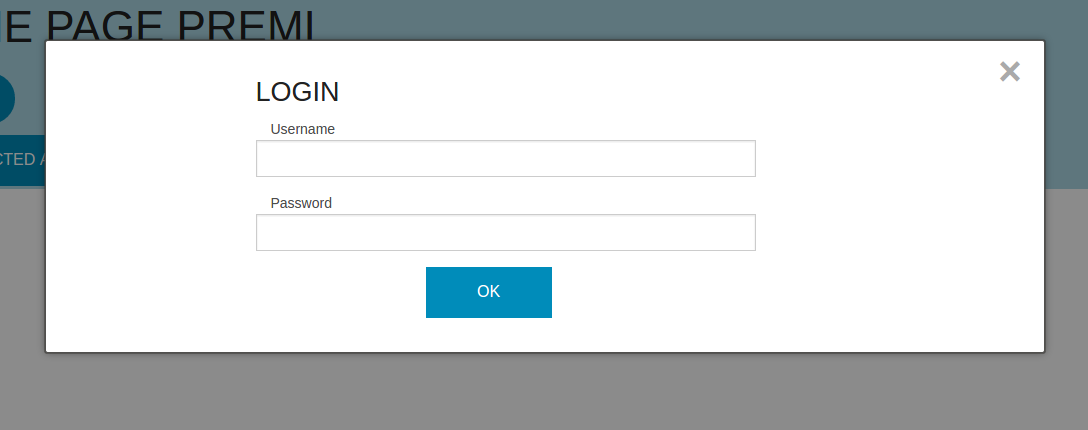
\includegraphics[scale=0.40] {img/MULogin.png}
	\caption{UC1 - Registrazione} 
\end{figure}

\noindent Una volta inseriti premere il pulsante \textbf{Login} situato sotto il form.

\section{Creazione di un Progetto}

Effettuata l'autenticazione è possibile cominciare a creare progetti.


\noindent Per creare un progetto selezionare dal menù in alto \textbf{New Project} e inserite un titolo per il progetto.


\section{Creazione di una Presentazione}

Una volta creato un progetto verrà automaticamente aperto l'editor che permette di creare le slide della presentazione.

\section{Creazione di un'Infografica}

Per creare un'infografica è sufficiente aprire un progetto e premere il pulsante \textbf{New Infographic}; dal menù laterale e verrà aperto l'editor con cui è possibile modificare l'infografica.

\section{Ricerca di un progetto}

È possibile fare una ricerca tra i progetti salvati da altri utenti.

\noindent Per fare ciò è sufficiente compilare il filtro di ricerca, presente sulla propria home page, e premere il pulsante \textbf{Search}.

Verrà visualizzata una lista di progetti che rispettano i parametri inseriti.

\noindent A questo punto basta selezionarne uno e scegliere la modalità di visualizzazione.
\newpage

\section{Ricerca di un progetto}
È possibile fare ricerche di progetti utilizzando come filtro l'username di un utente oppure il nome di un progetto.
\newline
Per eseguire una ricerca è sufficiente recarsi sulla home page tramite l'utilizzo del pulsante \textbf{PREMI} posto nell'angolo superiore sinistro dello schermo, scrivere la chiave di ricerca nell'apposita casella di testo, selezionare il filtro che si vuole utilizzare (Users o Project) e infine premere il tasto \textbf{Search}.

\begin{figure}[h] 
	\centering 
	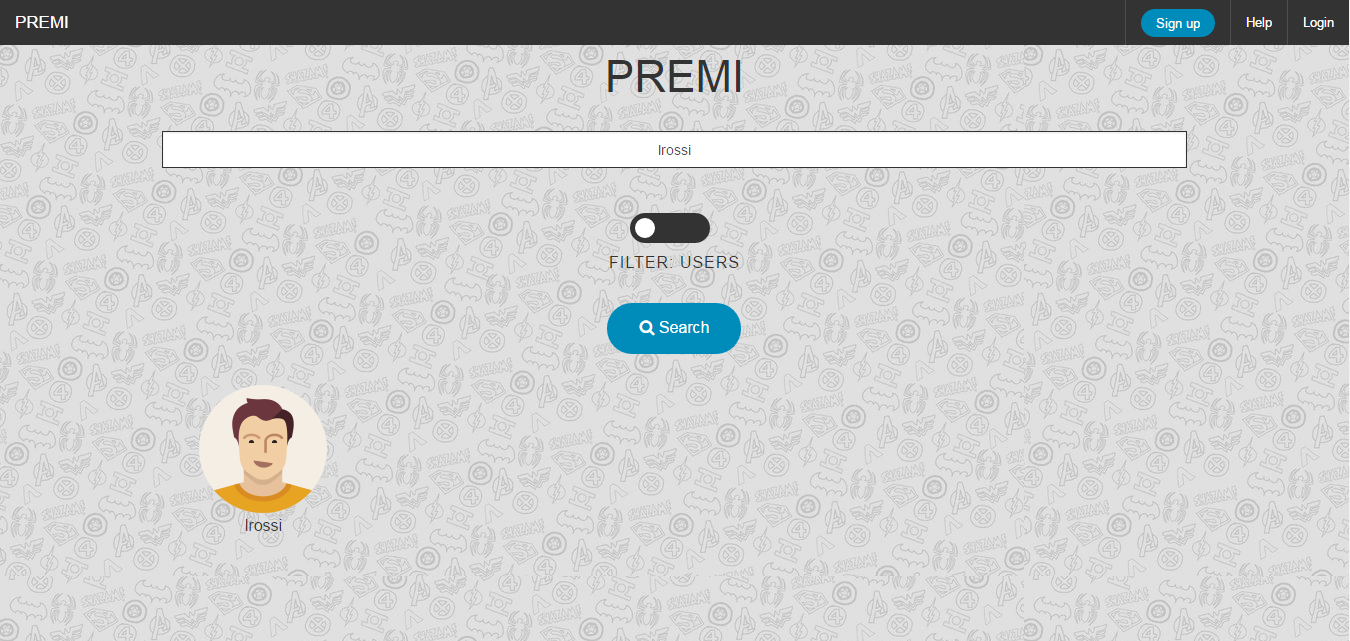
\includegraphics[scale=0.40] {img/ricerca.png}
	\caption{Ricerca} 
\end{figure}


\noindent I risultati della ricerca verranno mostrati sotto il pulsante \textbf{Search}, come mostrato nella figura sottostante.

\begin{figure}[h] 
	\centering 
	
\includegraphics[scale=0.40] {img/ricercaris.png}
	\caption{Risultati ricerca} 
\end{figure}
\newpage

\section{Creazione di un progetto}
Per creare un progetto un utente deve essere iscritto ed autenticato. Per accedere alla pagina di creazione di un progetto l'utente deve premere il pulsante azzurro \textbf{My Project} posto in alto a destra sullo schermo. Una volta premuto si caricherà la pagina corrispondente. A questo punto l'utente deve premere il pulsante verde \textbf{New Project} posto in alto a sinistra; si aprirà un pop-up\ped{G} nel quale viene richiesto di inserire il nome del progetto che si vuole creare. Una volta inserito il nome basterà premere il pulsante \textbf{OK}.


\noindent Una volta premuto il tasto \textbf{OK} il nuovo progetto sarà creato e aggiunto alla lista dei progetti dell'utente (vedi figura sottostante).


\begin{figure}[H] 
	\centering 
	
\includegraphics[scale=0.60] {img/projectlist}
	\caption{Lista dei progetti disponibili} 
\end{figure}

\section{Eliminazione di un progetto}
Per eliminare un progetto un utente deve essere iscritto ed autenticato. Per accedere alla pagina di eliminazione di un progetto l'utente deve premere il pulsante azzurro \textbf{My Project} posto in alto a destra sullo schermo. Una volta premuto si caricherà la pagina corrispondente. A questo punto l'utente deve selezionare il progetto da eliminare dalla lista dei progetti in alto a sinistra.
Una volta selezionato il progetto apparirà al centro dello schermo il titolo del progetto scelto,un'immagine di anteprima della prima slide del progetto e sotto a questa un menù. 

\begin{figure}[H] 
	\centering 
	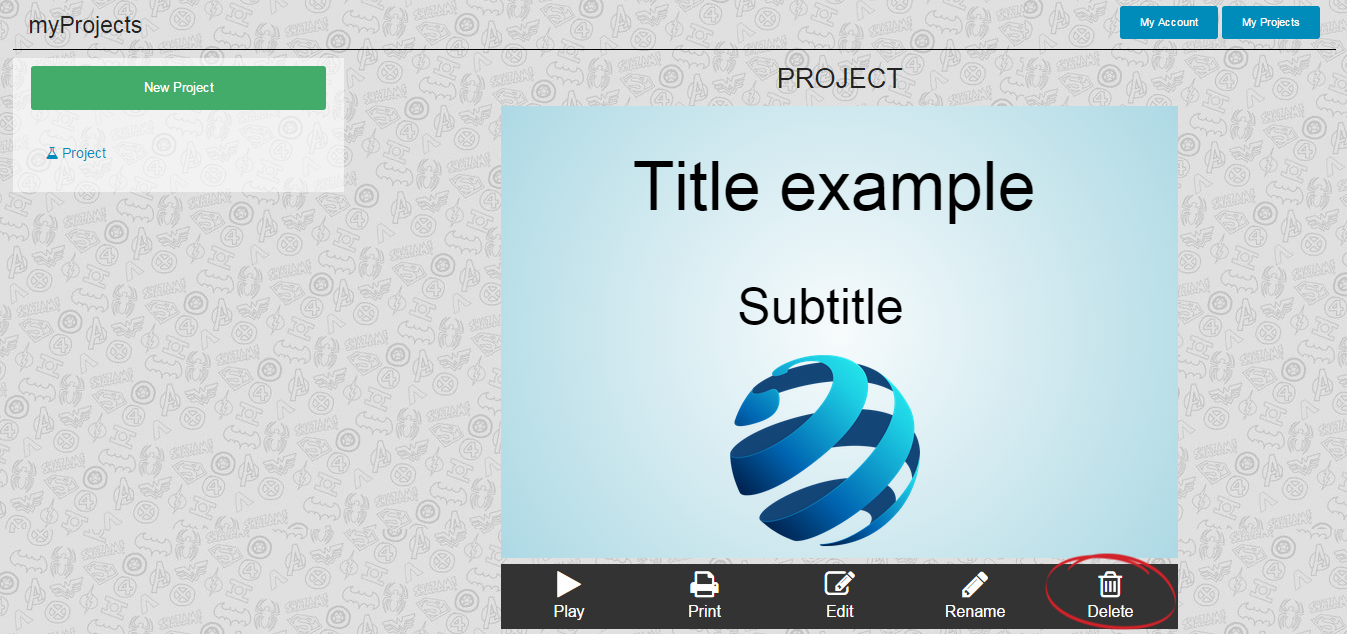
\includegraphics[scale=0.40] {img/elimina_pro.png}
	\caption{Eliminazione di un progetto} 
\end{figure}

Selezionando dal menù la voce \textbf{Delete} apparirà il seguente pop-up\ped{G}:

\begin{figure}[H] 
	\centering 
	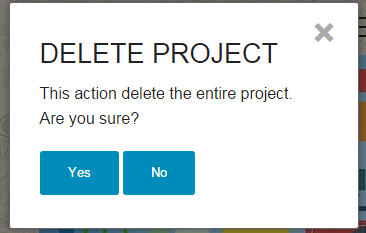
\includegraphics[scale=0.60] {img/del_project.png}
	\caption{Pop-up conferma eliminazione progetto} 
\end{figure}

\noindent Premendo il tasto \textbf{Yes} si confermerà l'eliminazione del progetto, premendo il tasto \textbf{No} il progetto non verrà eliminato.

\section{Rinominazione di un progetto}
Per rinominare un progetto un utente deve essere iscritto ed autenticato. Per accedere alla pagina di rinominazione di un progetto l'utente deve premere il pulsante azzurro \textbf{My Project} posto in alto a destra sullo schermo. Una volta premuto si caricherà la pagina corrispondente. A questo punto l'utente deve selezionare il progetto da rinominare dalla lista dei progetti in alto a sinistra.
Una volta selezionato il progetto apparirà al centro dello schermo il titolo del progetto scelto, un'immagine di anteprima della prima slide del progetto e sotto a questa un menù. 

\begin{figure}[H] 
	\centering 
	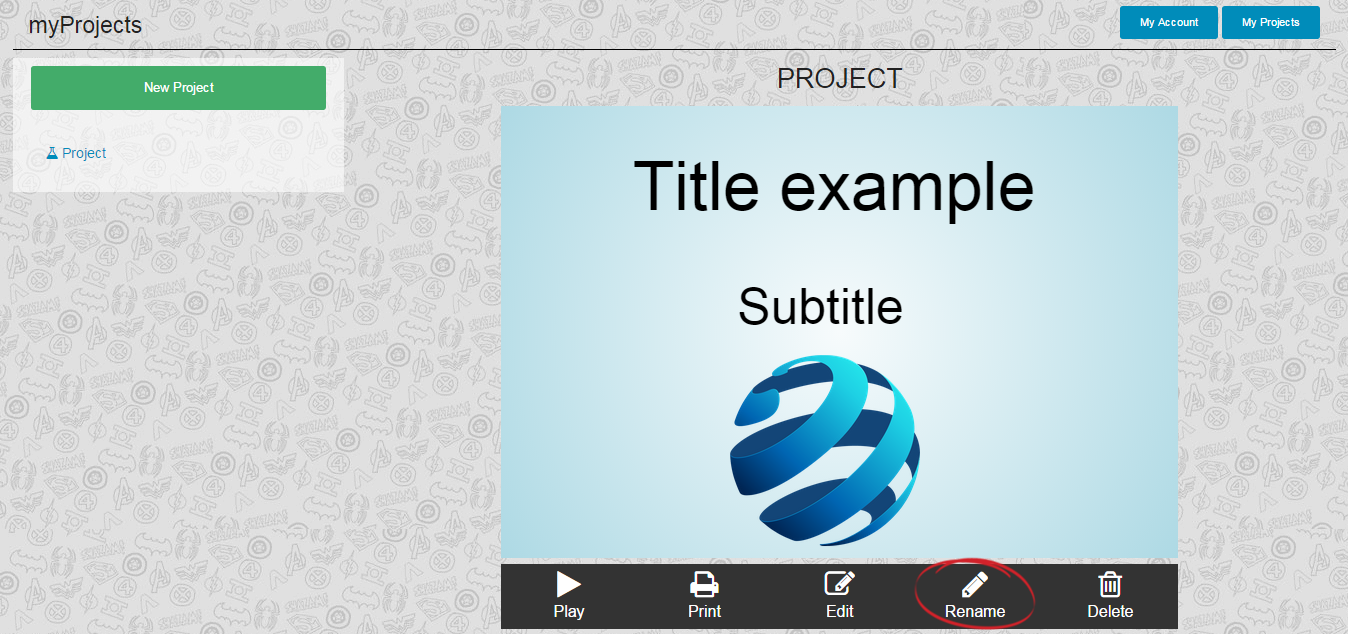
\includegraphics[scale=0.40] {img/rinomina_pro.png}
	\caption{Rinominazione di un progetto} 
\end{figure}

Selezionando dal menù la voce \textbf{Rename} apparirà il seguente pop-up\ped{G}:

\begin{figure}[H] 
	\centering 
	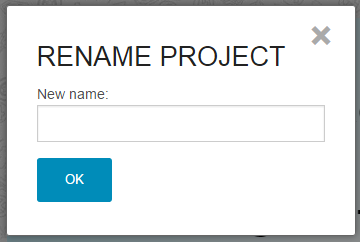
\includegraphics[scale=0.60] {img/rename_project.png}
	\caption{Pop-up di rinominazione di un progetto} 
\end{figure}

\noindent Per rinominare il progetto sarà sufficiente inserire nell'apposito spazio il nuovo nome che si desidera dare al progetto e successivamente confermare tramite il tasto \textbf{OK}. 

\section{Stampa ed esportazione di una presentazione}
Per stampare un progetto oppure per esportare il progetto in formato PDF\ped{G} un utente deve essere iscritto ed autenticato. Per accedere alla pagina di stampa ed esportazione di un progetto l'utente deve premere il pulsante azzurro \textbf{My Project} posto in alto a destra sullo schermo. Una volta premuto si caricherà la pagina corrispondente. A questo punto l'utente deve selezionare il progetto da stampare o esportare dalla lista dei progetti in alto a sinistra.
Una volta selezionato il progetto apparirà al centro dello schermo il titolo del progetto scelto, un'immagine di anteprima della prima slide\ped{G} del progetto e sotto a questa un menù. 

\begin{figure}[H] 
	\centering 
	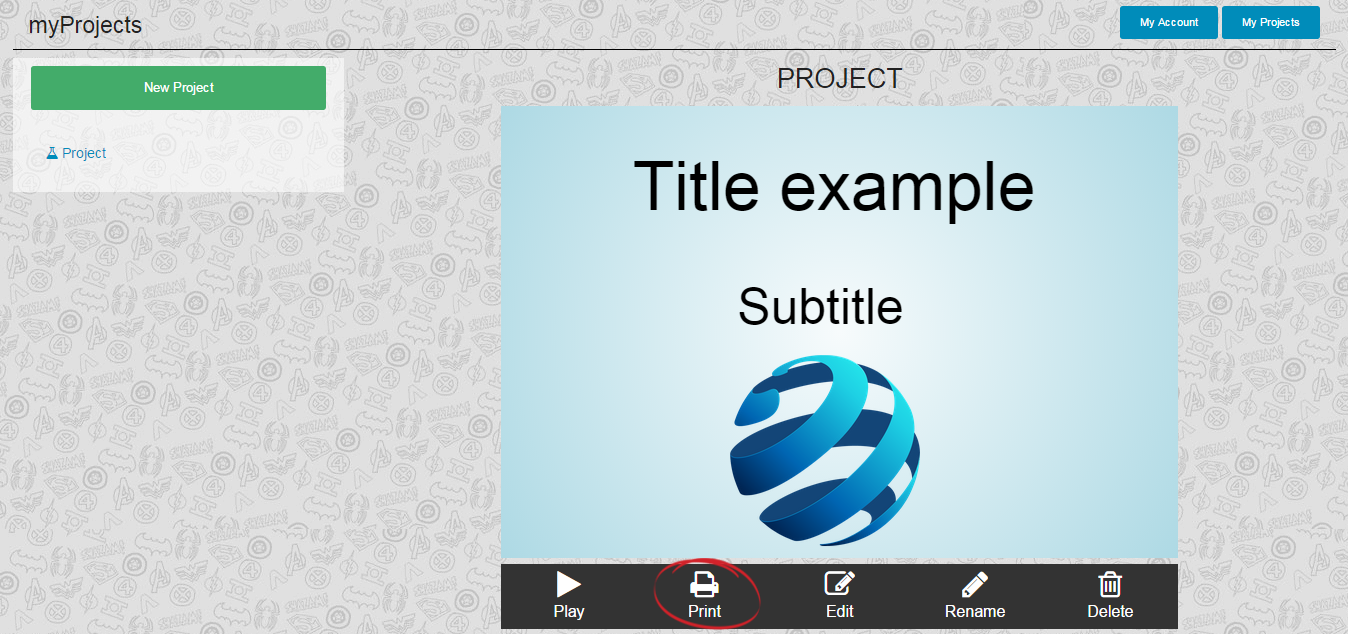
\includegraphics[scale=0.40] {img/stampa_pro.png}
	\caption{Stampa ed esportazione di un progetto} 
\end{figure}

\noindent Selezionando dal menù la voce \textbf{Print} si aprirà una nuova scheda dove verrà visualizzata l'intera presentazione come un'unica pagina web. Le slide\ped{G} verranno impaginate verticalmente una sotto l'altra nell'ordine in cui vengono visualizzate nella presentazione.

\begin{figure}[H] 
	\centering 
	
\includegraphics[scale=0.40] {img/print.png}
	\caption{Stampa ed esportazione di un progetto - Presentazione come un'unica pagina} 
\end{figure}

\subsection{Stampa di una presentazione}
\noindent Nel caso in cui si voglia stampare la presentazione è sufficiente utilizzare la funzione stampa presente nel browser\ped{G} che si sta utilizzando. Per ogni chiarimento in merito è consigliata la consultazione del manuale d'utilizzo del proprio browser\ped{G}. 

\subsection{Esportazione di una presentazione}
Nel caso in cui si voglia esportare la presentazione in formato PDF\ped{G} si dovrà utilizzare la funzionalità di stampa presente in Google Chrome\ped{G} e successivamente sfruttare la stampa su file. Di seguito verrà indicata la procedura da seguire, per questa guida è stata usata la versione 42 di Google Chrome\ped{G}. Una volta selezionata la funzionalità di stampa, apparirà la seguente schermata:

\begin{figure}[H] 
	\centering 
	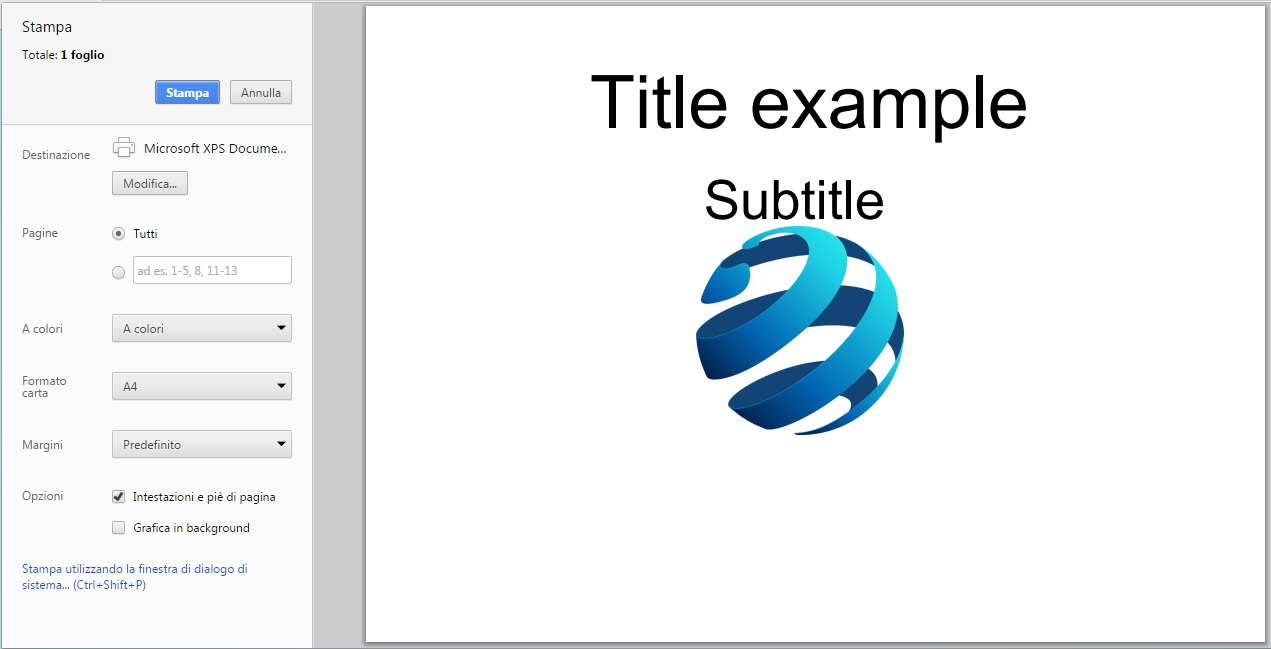
\includegraphics[scale=0.40] {img/print_google.png}
	\caption{Stampa ed esportazione di un progetto - Esportazione in formato PDF con Google Chrome} 
\end{figure}

\noindent Nel menù laterale di sinistra, a fianco alla voce \textit{Destinazione} selezionare il pulsante \textbf{Modifica...} e successivamente selezionare la voce \textit{Salva come PDF\ped{G}} (vedi figura sotto): 

\begin{figure}[H] 
	\centering 
	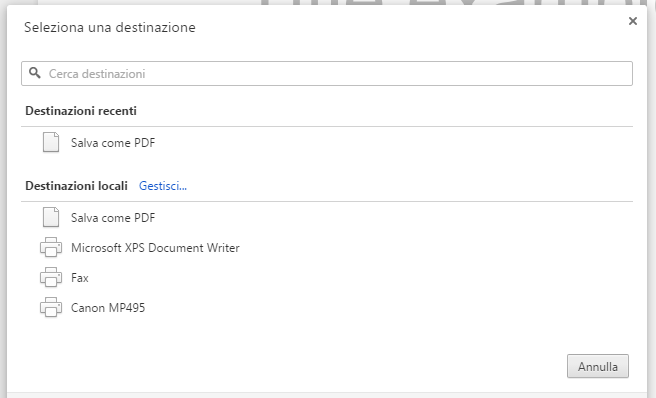
\includegraphics[scale=0.40] {img/salvacome.png}
	\caption{Stampa ed esportazione di un progetto - Settaggio stampa PDF con Google Chrome} 
\end{figure}

\noindent Una volta seguiti questi passi sarà sufficiente premere il pulsante di colore blu \textbf{Salva} e scegliere la destinazione di salvataggio della presentazione. 


\section{Creazione di una presentazione}
Per creare una presentazione è necessario prima selezionare il progetto dalla lista dei progetti disponibili. Una volta selezionato il progetto apparirà al centro dello schermo il titolo del progetto scelto, un'immagine di anteprima della prima slide\ped{G} del progetto e sotto a questa un menù. Selezionando dal menù la voce \textbf{Edit} si accederà alla pagina relativa alla creazione della presentazione, con le relative funzioni.

\begin{figure}[H] 
	\centering 
	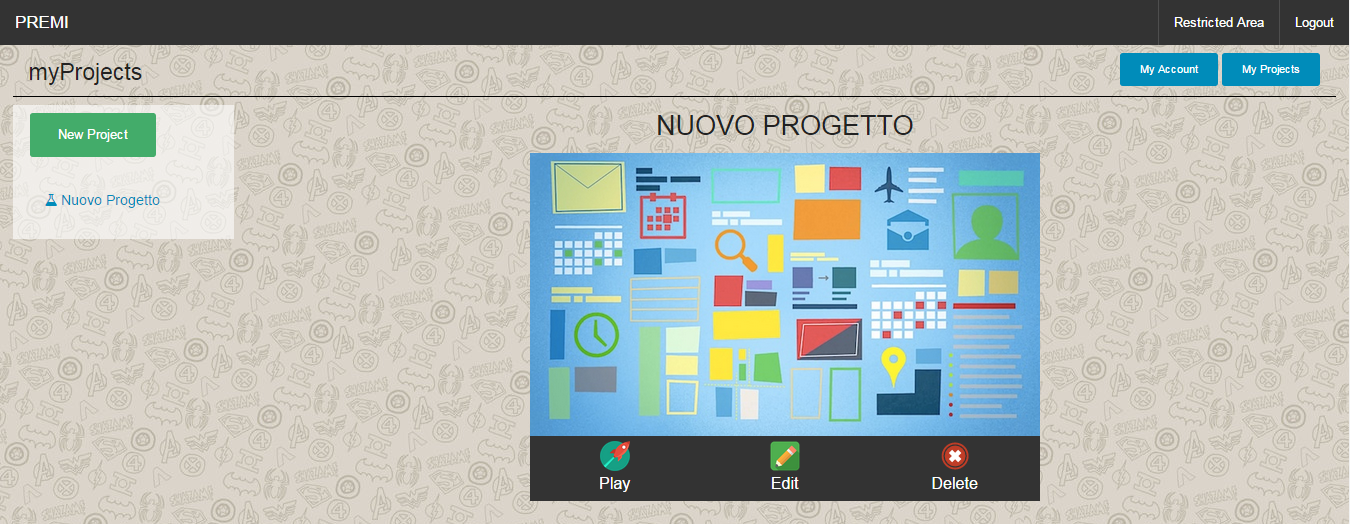
\includegraphics[scale=0.40] {img/presentazione.png}
	\caption{Creazione di una presentazione} 
\end{figure}
\newpage


\section{Editor presentazioni}
Di seguito vengono spiegati l'utilizzo degli strumenti di modifica delle presentazioni.

\subsection{Layout principale}
Una volta avviato l'editor delle presentazioni la pagina che appare si presenta semplice ed intuitiva. A sinistra si trova un menù verticale con tutti i pulsanti che permettono di modificare la slide corrente. Al centro dello schermo invece si trova lo spazio di gestione dei contenuti della slide, dove è possibile interagire con i contenuti.

\begin{figure}[H] 
	\centering 
	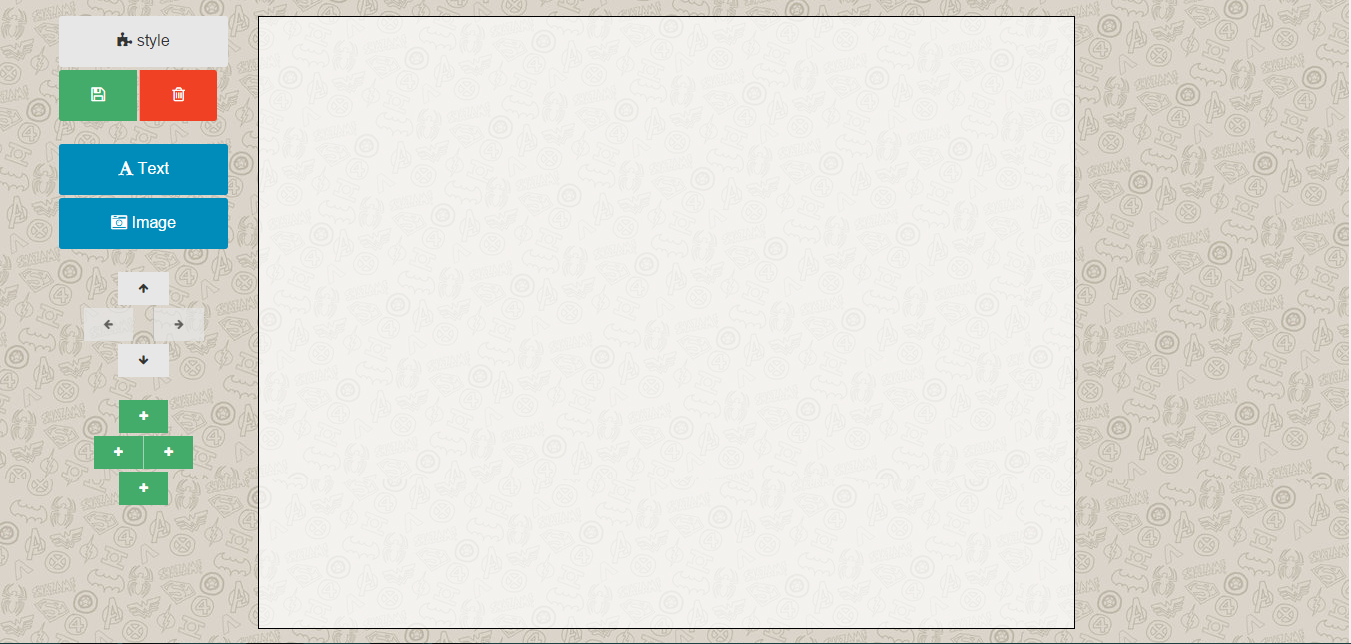
\includegraphics[scale=0.40] {img/layout_editor.png}
	\caption{Layout principale} 
\end{figure}

Di seguito verrà analizzato, dall'alto verso il basso, ciascun pulsante presente.

\subsection{Menù laterale}
\begin{itemize}
 \item \textbf{Style}\\
    Il pulsante \textbf{Style} permette di scegliere gli effetti di transizione e il tema da applicare alla slide. Una volta scelte le modifiche si deve confermare con il tasto \textbf{OK}.	
    \begin{figure}[H] 
    	\centering 
    	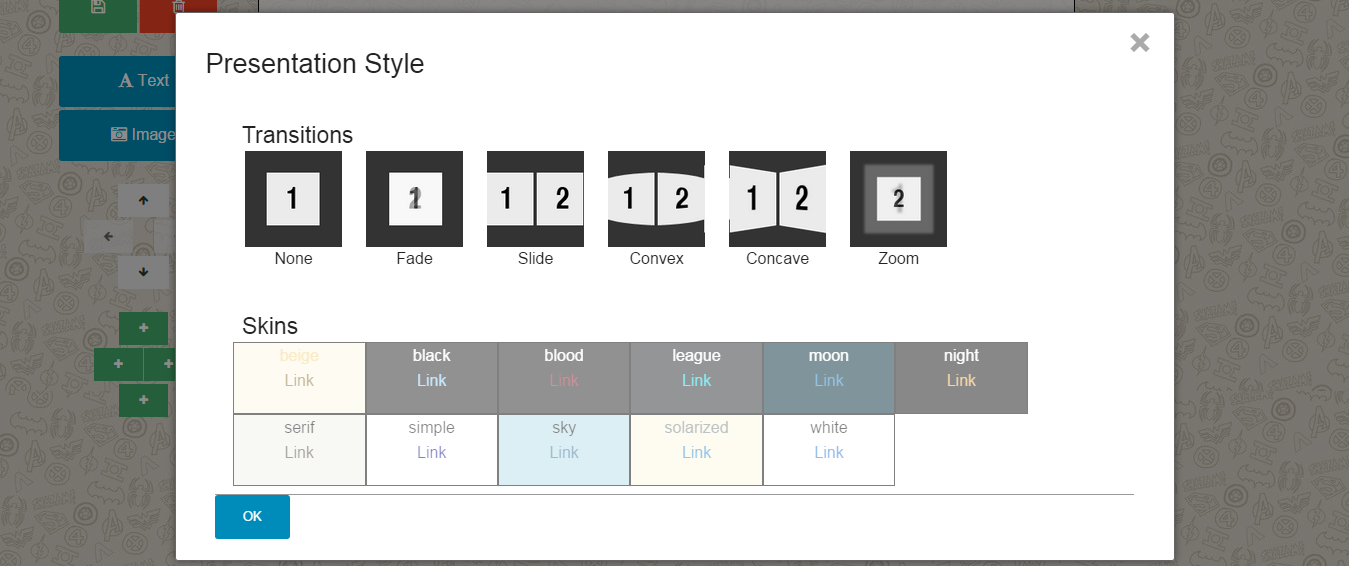
\includegraphics[scale=0.40] {img/editor_style.png}
    	\caption{Menù laterale - Style} 
    \end{figure}
	
 \item \textbf{Salva}\\
	Il pulsante di colore verde è il pulsante che permette di salvare le modifiche apportate alla slide. 	
	\begin{figure}[H] 
		\centering 
		
\includegraphics[scale=0.40] {img/editor_save.png}
		\caption{Menù laterale - Salva} 
	\end{figure}
	
	 \item \textbf{Elimina}\\
	 Il pulsante di colore rosso è il pulsante che permette di eliminare tutto il contenuto della slide corrente.  	
	 \begin{figure}[H] 
	 	\centering 
	 	
\includegraphics[scale=0.40] {img/editor_del.png}
	 	\caption{Menù laterale - Elimina} 
	 \end{figure}
	
 \item \textbf{Text}\\
    Il pulsante \textbf{Text} permette di inserire del testo nella slide. Una volta inserito il testo nell'apposita casella si deve confermare con il tasto \textbf{OK}.
    \begin{figure}[H] 
	\centering 
	
\includegraphics[scale=0.40] {img/editor_text.png}
	\caption{Menù laterale - Text} 
    \end{figure}
    
    
 \item \textbf{Image}\\
    Il pulsante \textbf{Image} permette di aggiungere un'immagine alla \gls{slide} corrente tra quelle già caricate o di caricarne un'altra presente sul file system dell'utente. Una volta scelta l'immagine questa verrà inserita automaticamente nella slide.
   \begin{figure}[H] 
	\centering 
	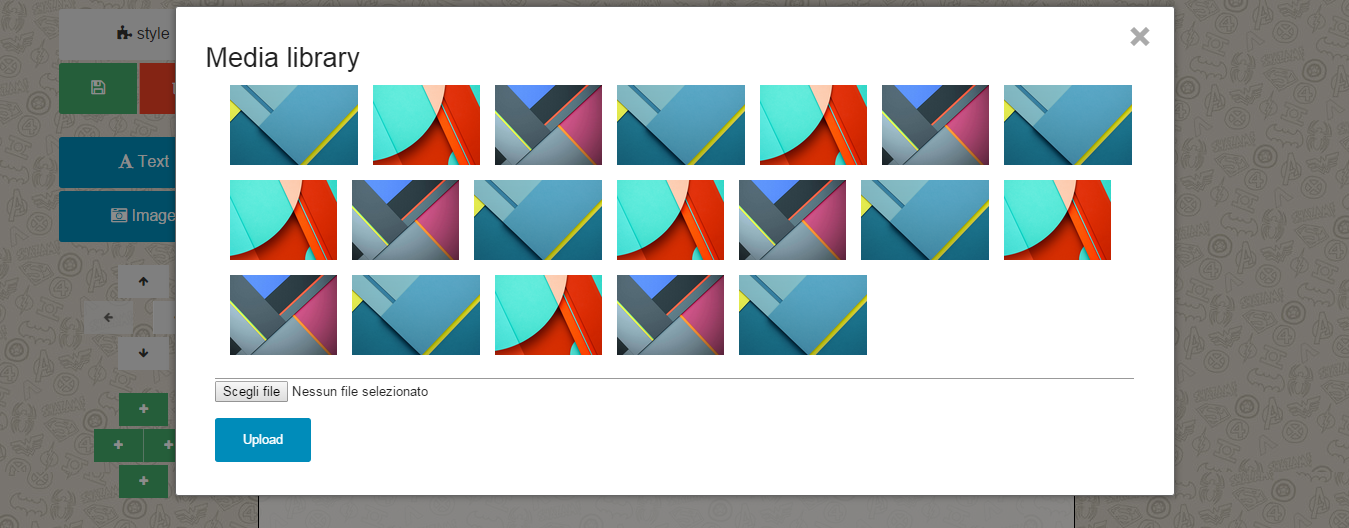
\includegraphics[scale=0.40] {img/editor_img.png}
	\caption{Menù laterale - Image} 
    \end{figure}
    
\newpage

  \item \textbf{Navigazione delle slide}\\
  I pulsanti freccia permettono di navigare tra le slide già create della presentazione. Ad ogni tasto corrisponde una direzione di spostamento.
  \begin{figure}[h] 
  	\centering 
  	
\includegraphics[scale=0.80] {img/editor_move.png}
  	\caption{Menù laterale - Aggiunta di una slide} 
  \end{figure}
 
 
 
\item \textbf{Aggiunta di una slide}\\
 Il pulsante con il simbolo \textbf{+} permette di aggiungere una nuova slide nella direzione corrispondente al pulsante premuto.
 \begin{figure}[h] 
 	\centering 
 	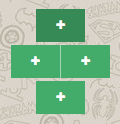
\includegraphics[scale=0.80] {img/editor_add.png}
 	\caption{Menù laterale - Aggiunta di una slide} 
 \end{figure}

\end{itemize}


\newpage

\subsection{Modifica di un componente}
Per modificare un componente è sufficiente selezionarlo nella \gls{slide} e modificarne gli attributi dal menù che comparirà sulla destra.

\subsubsection{Text}
La grandezza, la posizione e la rotazione della casella di testo possono essere modificate con il mouse tramite gli appositi punti di ancoraggio che compaiono una volta selezionato il testo. Il trascinamento in un angolo provoca una variazione della dimensione proporzionale tra larghezza ed altezza.

\begin{figure}[H] 
	\centering 
	
\includegraphics[scale=0.80] {img/text_anchor.png}
	\caption{Modifica di un componente - Modifica testo con mouse} 
\end{figure}

\noindent In alternativa si possono modificare le proprietà del testo dal menù laterale di destra, nel dettaglio:
		
		\begin{itemize}
			\item \textbf{ScaleX}: modifica la larghezza della casella di testo;
			\item \textbf{ScaleY}: modifica l'altezza della casella di testo;
			\item \textbf{Freccia verso l'alto}: sposta la casella di testo di un livello verso l'alto;
			\item \textbf{Freccia verso il basso}: sposta la casella di testo di un livello verso il basso;
			\item \textbf{Delete}: elimina la casella di testo;
			\item \textbf{Text}: modifica il testo contenuto nella casella di testo;
			\item \textbf{Tasto B}: modifica lo stile del testo in BOLD;
			\item \textbf{Tasto I}: modifica lo stile del testo in ITALIC;
			\item \textbf{Tasto U}: modifica lo stile del testo in UNDERLINE;
			\item \textbf{Size}: modifica la grandezza del testo;
			\item \textbf{Select Font}: modifica il font del testo.
		\end{itemize}
		 \begin{figure}[h] 
		    \centering 
		    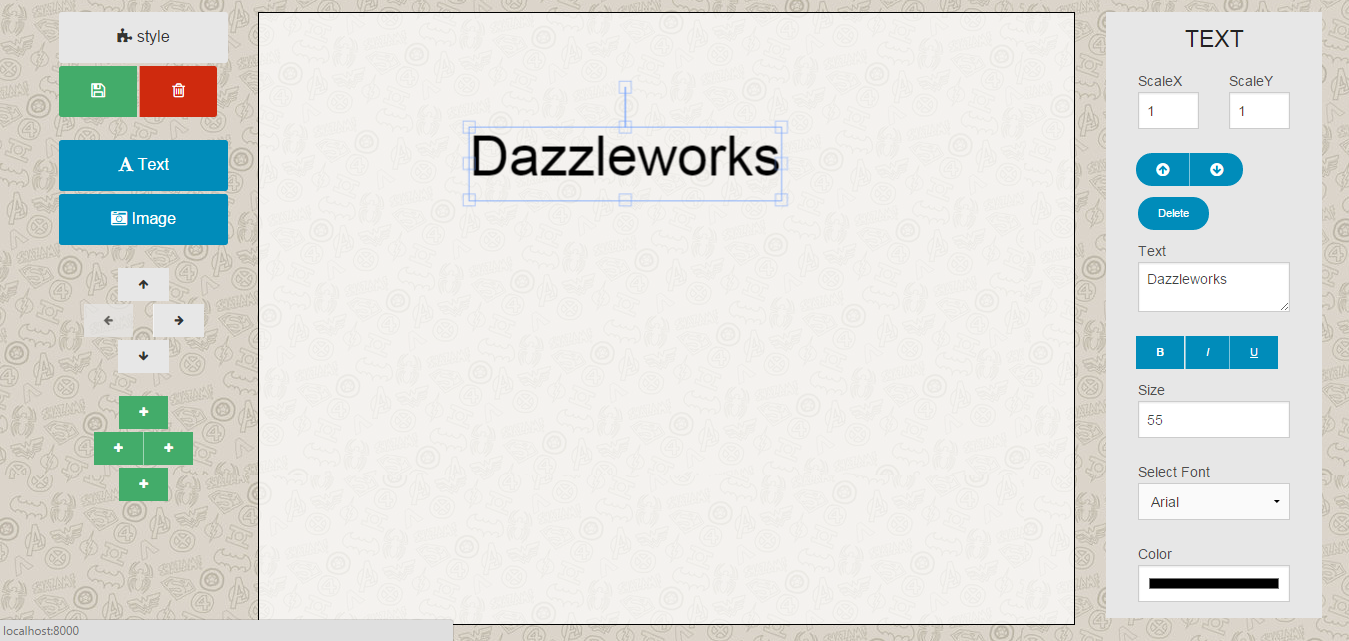
\includegraphics[scale=0.40] {img/text_edit.png}
		    \caption{\gls{Slide} Editor - Modifica testo da menù} 
		\end{figure}
		
		
\newpage 

\subsubsection{Image}
La grandezza, la posizione e la rotazione dell'immagine possono essere modificate con il mouse tramite gli appositi punti di ancoraggio che compaiono una volta selezionata l'immagine. Il trascinamento in un angolo provoca una variazione della dimensione proporzionale tra larghezza ed altezza.

\begin{figure}[H] 
	\centering 
	
\includegraphics[scale=0.80] {img/img_anchor.png}
	\caption{Modifica di un componente - Modifica immagine con mouse} 
\end{figure}

\noindent In alternativa si possono modificare le proprietà dell'immagine dal menù laterale di destra, nel dettaglio:

		\begin{itemize}
			\item \textbf{ScaleX}: modifica la larghezza dell'immagine;
			\item \textbf{ScaleY}: modifica l'altezza dell'immagine;
			\item \textbf{Freccia verso l'alto}: sposta l'immagine di un livello verso l'alto;
			\item \textbf{Freccia verso il basso}: sposta l'immagine di un livello verso il basso;
			\item \textbf{Delete}: elimina l'immagine;
		\end{itemize}
		
\begin{figure}[H] 
	\centering 
	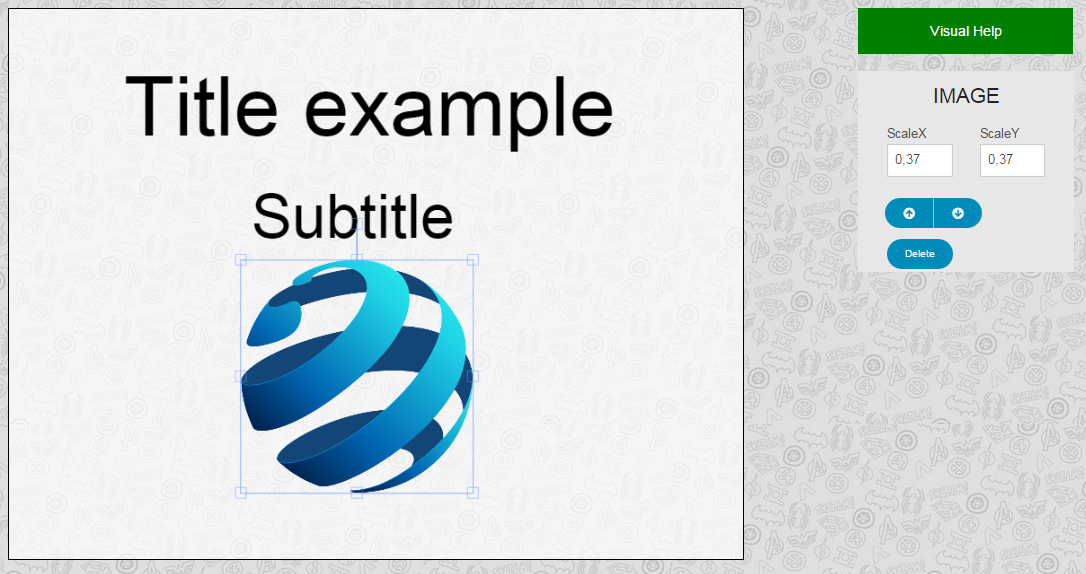
\includegraphics[scale=0.40] {img/img_edit.png}
	\caption{\gls{Slide} Editor - Modifica immagine da menù} 
\end{figure}	



\newpage


\section{Visualizzazione presentazioni}
\noindent
Per entrare in modalità visualizzazione di una presentazione è necessario entrare nel progetto ad essa asciato e premere il bottone play. 

All'interno di una presentazione sono possibili le seguenti azioni:

\begin{itemize}
 \item \textbf{spostamento tra slides}: \\disponibile attraverso dei tasti freccia in basso a destra o mediante i tasti freccia della tastiera.
 \item \textbf{passare in modalità presentatore}: \\disponibile attraverso la pressione del tasto '\textbf{S}' della tastiera (S sta per Speaker View).
  \item \textbf{pausa esposizione}: \\disponibile attraverso la pressione del tasto '\textbf{B}' della tastiera (B sta per Blind). In questa modalità la presentazione si oscura, permettendo al presentatore di fare una pausa.
  \item \textbf{visualizzazione dell'indice}: \\disponibile attraverso la pressione del tasto '\textbf{esc}' della tastiera. In questa modalità è possibile vedere la matrice completa di tutte le \gls{slide} che compongono la presentazione.

  \end{itemize}

\newpage

\section{Segnalazione degli errori}
Per la segnalazione di eventuali errori l'utente dovrà spedire una mail all'indirizzo \textbf{\textit{support@dazzleworks.it}} con la seguente formattazione:
\begin{itemize}
	\item \textbf{Oggetto}: pagina o pulsante che provoca l'errore o un comportamento diverso da quanto descritto nel \textit{manuale utente};
	
	\item \textbf{Testo della mail}: una descrizione, il più precisa e dettagliata possibile sull'errore riscontrato e il nome utente del profilo utilizzato dall'utente;
	
	\item \textbf{Allegati}: se possibile allegare uno screenshot\ped{G} della pagina nella quale l'errore si verifica.
\end{itemize}

\noindent Ogni segnalazione verrà visionata e presa in carico nel minor tempo possibile, verrà infine spedita una mail di risposta all'utente con le eventuali procedure da adottare per evitare l'errore o con una segnalazione di avvenuta correzione di quest'ultimo.
\newpage


\section{Glossario}
\paragraph{B}
\begin{itemize}
	\item[] \textbf{Browser}: un browser è un programma che consente di visualizzare i contenuti delle pagine web e di interagire con esse.
\end{itemize}

\newpage


\paragraph{F}
\begin{itemize}
	\item[] \textbf{Facebook}: servizio di rete sociale lanciato nel febbraio del 2004. 

	\item[] \textbf{File system}: indica informalmente un meccanismo con il quale i file sono posizionati e organizzati o su un dispositivo di archiviazione o su una memoria di massa, come ad esempio un disco rigido.
\end{itemize}
\newpage

\paragraph{G}
\begin{itemize}
	\item[] \textbf{Google}: è un motore di ricerca per Internet il cui dominio è stato registrato il 15 settembre 1997.
	\item[] \textbf{Google Chrome}: è un browser\ped{G} sviluppato da Google\ped{G}.
\end{itemize}
\newpage

\paragraph{H}
\begin{itemize}
	\item[] \textbf{HTML5}: linguaggio di markup\ped{G} per la strutturazione delle pagine web, da ottobre 2014 pubblicato come W3C Recommendation.
\end{itemize}
\newpage

\paragraph{I}
\begin{itemize}
	\item[] \textbf{Internet Explorer}: è un browser web grafico proprietario sviluppato da Microsoft e incluso in Windows\ped{G} a partire dal 1995.
\end{itemize}
\newpage


\paragraph{L}
\begin{itemize}
	\item[] \textbf{Linguaggio di markup}: un linguaggio di markup è un insieme di regole che descrivono i meccanismi di rappresentazione (strutturali, semantici o presentazionali) di un testo che, utilizzando convenzioni standardizzate, sono utilizzabili su più supporti.
\end{itemize}
\newpage

\paragraph{M}
\begin{itemize}
	\item[] \textbf{Mozilla Firefox}: è un web browser open source multipiattaforma prodotto da Mozilla Foundation.
\end{itemize}
\newpage

\paragraph{O}
\begin{itemize}
	\item[] \textbf{Opera}: è un browser web freeware e multipiattaforma prodotto da Opera Software.
\end{itemize}
\newpage

\paragraph{S}
\begin{itemize}
	\item[] \textbf{Screenshot}: lo screenshot è il risultato della cattura (istantanea) di ciò che è visualizzato sul monitor del computer.
	\item[] \textbf{Software}: è l'informazione o le informazioni utilizzate da uno o più sistemi informatici e memorizzate su uno o più supporti informatici. Tali informazioni possono essere quindi rappresentate da uno o più programmi, oppure da uno o più dati, oppure da una combinazione delle due.
\end{itemize}
\newpage


\paragraph{P}
\begin{itemize}
	\item[] \textbf{PDF}:  è un formato di file basato su un linguaggio di descrizione di pagina sviluppato da Adobe Systems nel 1993 per rappresentare documenti in modo indipendente dall'hardware e dal software utilizzati per generarli o per visualizzarli.
	\item[] \textbf{Pop-up}: sono degli elementi dell'interfaccia grafica, quali finestre o riquadri, che compaiono automaticamente durante l'uso di un'applicazione ed in determinate situazioni, per attirare l'attenzione dell'utente.
\end{itemize}
\newpage

\paragraph{S}
\begin{itemize}
	\item[] \textbf{Safari}: è un browser web sviluppato da Apple Inc.
	\item[] \textbf{Slide}: diapositiva digitale.
\end{itemize}
\newpage

\paragraph{W}
\begin{itemize}
	\item[] \textbf{Windows}: è una famiglia di ambienti operativi e sistemi operativi dedicati ai personal computer, alle workstation, ai server e agli smartphone.
\end{itemize}
\newpage

\paragraph{Acronimi}
\begin{itemize}
	\item[] \textbf{PDF}: Portable Document Format;
	\item[] \textbf{W3C}: World Wide Web Consortium.
\end{itemize}
\newpage

%\newpage

% ...

%\printglossaries

\end{document}
